\paragraph{}
Having a few error indicator may not be a good story as some of them can be correlated to each others and contribute little to decided whether a cell need to be refined.
As a result, some statistical technique is required to find out a set of most significant variables.

\paragraph{}
Support Vector Machine(SVM) is a popular method in solving classification in machine learning.
The data set called training set includes both criteria and the classifications.
SVM can be trained to solve the linearly separable problem and non-linearly separable upon some special technique.


%   ----    %
\subsection{Training Set}
\paragraph{}
The training set is determined by a numerical example in fig.~\ref{adap_fig:svm_train} \cite{Duval2018}.
\begin{figure}[!ht]
    \centering
    \begin{subfigure}[b]{0.5\linewidth}
        \scalebox{0.7}{
            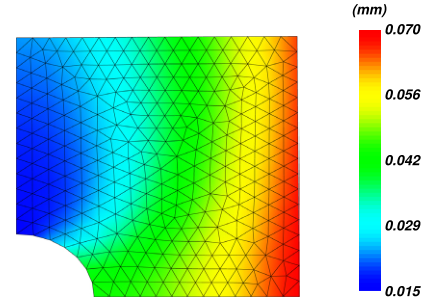
\includegraphics{adaptivity/images/adap_svm_train_0.png}
        }
        \caption{Mesh and displacement field before refinement}
    \end{subfigure}
    \begin{subfigure}[b]{0.5\linewidth}
        \scalebox{0.7}{
            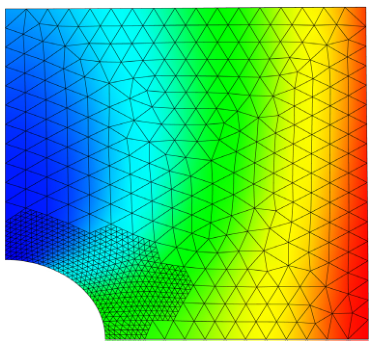
\includegraphics{adaptivity/images/adap_svm_train_1.png}
        }
        \caption{Mesh and displacement field after refinement}
    \end{subfigure}
    \caption{Mesh refinement for square plate with circular hole \cite{Duval2018}}
    \label{adap_fig:svm_train}
\end{figure}


\paragraph{}
With the same example, an uniform mesh of quadtree is conducted and the same region is marked as refined as shown in fig.~\ref{adap_fig:svm_train_my}
\begin{figure}[!ht]
    \centering
    \scalebox{0.5}{
        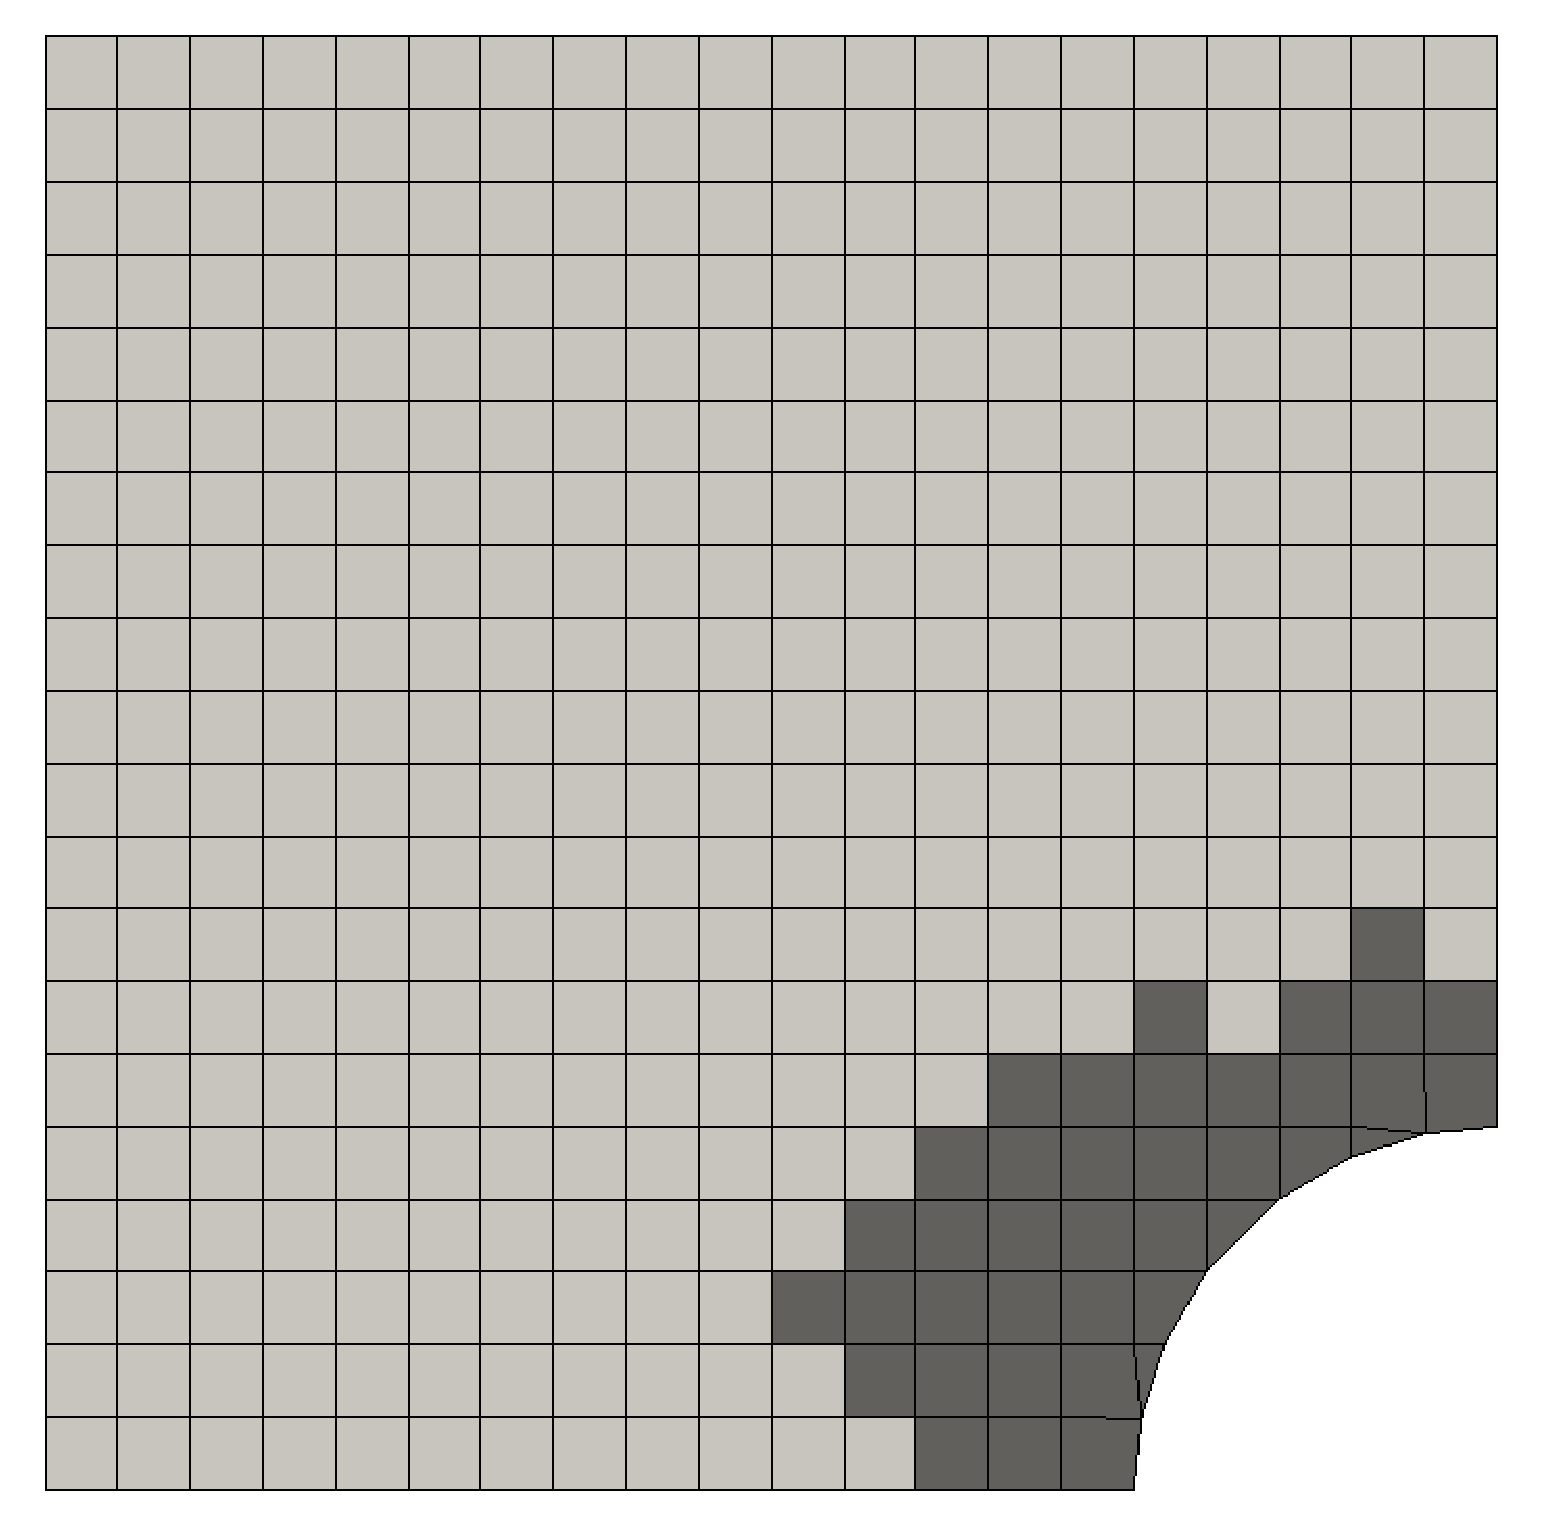
\includegraphics{adaptivity/images/adap_svm_train_my.eps}
    }
    \caption[Training data for SVM]{Training data for SVM: Cells in black is marked as refined.}
    \label{adap_fig:svm_train_my}
\end{figure}
Criteria taken into consideration are: 
\begin{enumerate}
    \item Area of the cell
    \item Minimal angle formed by the intersecting lines connected by scaling center and adjacent polygon vertexes
    \item Eigenvalue error indicator for displacement
    \item Eigenvalue error indicator for stress
\end{enumerate}
All data are normalized into the range of $[0,1]$, cell that need to be refined are labeled as $1$ and the rest are labeled as $0$.
Radial basis function with $\sigma^2=\frac{1}{2}$ is adopted as kernel function.
Half of the training data (192 out of 383) are used to train the model and the reset are used as a cross validation.
A score of $0.9581$ indicate the model may be valid.





\pagebreak